\documentclass[12pt,a4paper]{article}

% ---------- Idioma y codificación ----------
\usepackage[utf8]{inputenc}
\usepackage[T1]{fontenc}
\usepackage{mathpazo}
% Si tu distribución no tiene instalado el idioma español, esta línea evita
% que la compilación falle (instalá "babel-spanish" para tenerlo completo).
\IfFileExists{spanish.ldf}
  {\usepackage[spanish,es-nodecimaldot,es-noshorthands]{babel}}
  {\usepackage[english]{babel}}
% Nota: la opción es-noshorthands (arriba) desactiva los shorthands "<" y ">"
% de babel-spanish, que de otro modo rompen la sintaxis de flechas de TikZ
% (">={...}").

% ---------- Página ----------
\usepackage[a4paper,top=3cm,bottom=2.5cm,left=2.5cm,right=2.5cm,headheight=1.5cm,headsep=0.8cm]{geometry}

% ---------- Utilidades ----------
\usepackage{graphicx}
\usepackage{fancyhdr}
\usepackage{lastpage}          % necesario para \pageref{LastPage}
\usepackage{xcolor}
\usepackage{enumitem}
\usepackage{tikz}
\usetikzlibrary{positioning,shapes.geometric,arrows.meta,calc,fit,backgrounds}
\usepackage[hidelinks]{hyperref}
\usepackage{titlesec}
\usepackage{float}
\usepackage{booktabs}
\usepackage{longtable}
\usepackage{amsmath}
\usepackage{amssymb}
\usepackage{listings}
\usepackage[numbers]{natbib}
\bibliographystyle{unsrtnat}
\newcommand{\sectionbreak}{\clearpage}

% ---------- Estilo para código Verilog ----------
\definecolor{codegray}{gray}{0.96}
\definecolor{codekw}{RGB}{0,90,160}
\definecolor{codecom}{RGB}{100,120,100}
\definecolor{codestr}{RGB}{160,60,60}
\definecolor{codenum}{gray}{0.45}

\lstdefinestyle{verilog}{
  language=Verilog,
  backgroundcolor=\color{codegray},
  basicstyle=\ttfamily\scriptsize,
  keywordstyle=\color{codekw}\bfseries,
  commentstyle=\color{codecom}\itshape,
  stringstyle=\color{codestr},
  numbers=left,
  numberstyle=\tiny\color{codenum},
  numbersep=8pt,
  showstringspaces=false,
  breaklines=true,
  breakatwhitespace=true,
  frame=single,
  rulecolor=\color{gray!40},
  framesep=4pt,
  xleftmargin=16pt,
  tabsize=4,
  captionpos=b,
  columns=fullflexible,
  morekeywords={always,posedge,negedge,localparam,parameter,logic,endcase,
                signed,unsigned,task,endtask,function,endfunction,initial,
                integer,timescale,display,finish,random,time,clog2,signed}
}
\lstset{style=verilog}
\renewcommand{\lstlistingname}{Código}

% ============================================================
%  >>>>>>>>>>  DATOS DEL TRABAJO: EDITAR ACÁ  <<<<<<<<<<
% ============================================================
\newcommand{\Titulo}{Trabajo Práctico N°1: ALU}
\newcommand{\Subtitulo}{Diseño, implementación y verificación de una ALU parametrizable en FPGA}
\newcommand{\Materia}{Arquitectura de Computadoras}
\newcommand{\Institucion}{Facultad de Ciencias Exactas, Físicas y Naturales - Universidad Nacional de Córdoba}
\newcommand{\Carrera}{Ingeniería en Computación}
%\newcommand{\Fecha}{\today}

% Integrantes: una línea \persona{...} por cada uno
\newcommand{\Integrantes}{%
  \persona{Brigido, Tomás Andrés}{Legajo 38481096}%
  \persona{Tosolini, Agustín}{Legajo 42332698}%
}

% Docentes
\newcommand{\Docentes}{%
  \persona{Pereyra, Martin}{}%
}

% Repositorio: dejar vacío {} para que NO aparezca en la carátula
\newcommand{\Repositorio}{}

% Logos del encabezado
\newcommand{\LogoIzquierdo}{./logos/unc.png}
\newcommand{\LogoDerecho}{./logos/fcefyn.png}
\newcommand{\AlturaLogo}{3.0cm}
% ============================================================


% ---------- Maquinaria interna (no hace falta tocar) ----------
\newcommand{\ponerlogo}[1]{%
  \IfFileExists{#1}{%
    \includegraphics[height=\AlturaLogo,keepaspectratio]{#1}%
  }{%
    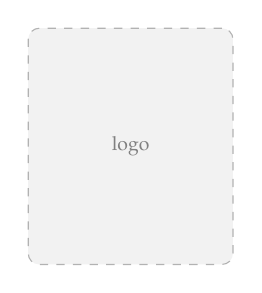
\begin{tikzpicture}
      \node[draw=gray!60,dashed,fill=gray!10,rounded corners,
            minimum height=\AlturaLogo,minimum width=2.6cm,
            font=\scriptsize\color{gray}] {logo};
    \end{tikzpicture}%
  }%
}

% Estilo de la carátula: sin encabezado (los logos van dentro de la página)
\fancypagestyle{caratula}{%
  \fancyhf{}
  \renewcommand{\headrulewidth}{0pt}
  \renewcommand{\footrulewidth}{0pt}
}

% Resto del documento: sólo el número de página al pie, SIN logos
\fancypagestyle{plain}{%
  \fancyhf{}
  \fancyfoot[C]{\small Página \thepage\ de \pageref{LastPage}}
  \renewcommand{\headrulewidth}{0pt}
  \renewcommand{\footrulewidth}{0pt}
}
\pagestyle{plain}

\newcommand{\persona}[2]{%
  \textbf{#1}%
  \ifx\relax#2\relax\else{\ \small(#2)}\fi\\[0.25em]
}

\setlength{\emergencystretch}{3em}
\hyphenpenalty=1000
\setlength{\parskip}{0.6em}
\setlength{\parindent}{0pt}


% ============================================================
\begin{document}

% ------------------------- CARÁTULA -------------------------
\thispagestyle{caratula}
\begin{center}
  % --- Logos: aparecen únicamente en esta página
  \noindent\makebox[\textwidth]{%
    \ponerlogo{\LogoIzquierdo}\hfill\ponerlogo{\LogoDerecho}%
  }\\[0.35cm]
  \rule{\textwidth}{0.4pt}

  \vspace{1.2cm}

  {\large \Institucion \par}
  {\normalsize \Carrera \par}

  \vspace{1.5cm}
  \rule{\textwidth}{1.2pt}\\[0.6cm]
  {\Huge\bfseries \Titulo \par}
  \vspace{0.4cm}
  \ifx\Subtitulo\empty\else{\Large \Subtitulo \par}\vspace{0.3cm}\fi
  \rule{\textwidth}{1.2pt}

  \vspace{0.8cm}
  {\large \textit{\Materia} \par}

  \vspace{2cm}
  {\large\bfseries Integrantes\par}
  \vspace{0.4cm}
  \Integrantes

  \vspace{1.2cm}
  {\large\bfseries Docente\par}
  \vspace{0.4cm}
  \Docentes

  \vfill

  %{\large \Fecha \par}
  \vspace{1cm}
\end{center}

\newpage

% --------------------- ÍNDICE ---------------------
\tableofcontents
\newpage

% ============================================================
\section{Introducción}
% ============================================================

% ============================================================
\section{Especificación}
% ============================================================

\subsection{Repertorio de operaciones}

La Tabla~\ref{tab:ops} reproduce el conjunto de operaciones exigido por el
enunciado. Los códigos corresponden al campo \texttt{funct} de las
instrucciones tipo R de MIPS, lo que facilita la reutilización posterior de este
módulo dentro de un procesador segmentado.

\begin{table}[H]
  \centering
  \begin{tabular}{llll}
    \toprule
    \textbf{Operación} & \textbf{Código} & \textbf{Expresión} & \textbf{Tipo} \\
    \midrule
    ADD & \texttt{100000} & $A + B$                     & Aritmética \\
    SUB & \texttt{100010} & $A - B$                     & Aritmética \\
    AND & \texttt{100100} & $A \;\&\; B$                & Lógica bit a bit \\
    OR  & \texttt{100101} & $A \;|\; B$                 & Lógica bit a bit \\
    XOR & \texttt{100110} & $A \oplus B$                & Lógica bit a bit \\
    NOR & \texttt{100111} & $\sim(A \;|\; B)$           & Lógica bit a bit \\
    SRA & \texttt{000011} & $A \ggg B[3{:}0]$           & Desplazamiento \\
    SRL & \texttt{000010} & $A \gg B[3{:}0]$            & Desplazamiento \\
    \midrule
    \multicolumn{2}{l}{\textit{cualquier otro código}} & $0$ & Caso por defecto \\
    \bottomrule
  \end{tabular}
  \caption{Operaciones implementadas y su codificación.}
  \label{tab:ops}
\end{table}

Obsérvese que los seis bits del selector permiten $2^6 = 64$ combinaciones, de
las cuales sólo 8 corresponden a operaciones definidas. Las 56 restantes se
resuelven en la rama \texttt{default}, que fuerza la salida a cero. Esta
decisión tiene dos consecuencias relevantes: cierra la especificación de la
función combinacional (no queda ningún caso sin definir) y, como se verá en la
Sección~\ref{sec:case}, evita la inferencia accidental de un \emph{latch} en el
bloque operacional.

\subsection{Interfaz del módulo}


% ============================================================
\section{Implementación de la ALU}
% ============================================================

\subsection{Observaciones sobre la parametrización}

% ============================================================
\section{Banco de pruebas}
% ============================================================

% Solo descripccion de capturas sin entrar en detalles de los testbenchs

% ============================================================
\begin{thebibliography}{9}

\bibitem{ieee1364}
IEEE Computer Society.
\emph{IEEE Standard for Verilog Hardware Description Language (IEEE Std 1364-2005)},
IEEE, 2006.

\bibitem{xilinx7series}
Xilinx Inc.
\emph{7 Series FPGAs Configurable Logic Block --- User Guide (UG474)},
Xilinx, 2016.

\bibitem{vivadosynth}
Xilinx Inc.
\emph{Vivado Design Suite User Guide: Synthesis (UG901)},
Xilinx, 2021.

\bibitem{vivadosim}
Xilinx Inc.
\emph{Vivado Design Suite User Guide: Logic Simulation (UG900)},
Xilinx, 2021.

\bibitem{pattersonhennessy}
D. A. Patterson y J. L. Hennessy.
\emph{Computer Organization and Design: The Hardware/Software Interface},
5\textsuperscript{a} ed., Morgan Kaufmann, 2013.

\bibitem{chusmith}
M. D. Ciletti.
\emph{Advanced Digital Design with the Verilog HDL},
2\textsuperscript{a} ed., Pearson, 2010.

\bibitem{cummings}
C. E. Cummings.
\emph{``full\_case parallel\_case'', the Evil Twins of Verilog Synthesis},
SNUG Boston, 1999.

\end{thebibliography}

\end{document}